\subsection*{Venneliste}
Venneliste inddeles i to boundaryklasser og en fælles controlklasse, som fremgår af \autoref{fig:MVCVenneliste}. 

\begin{figure} [H]
\centering
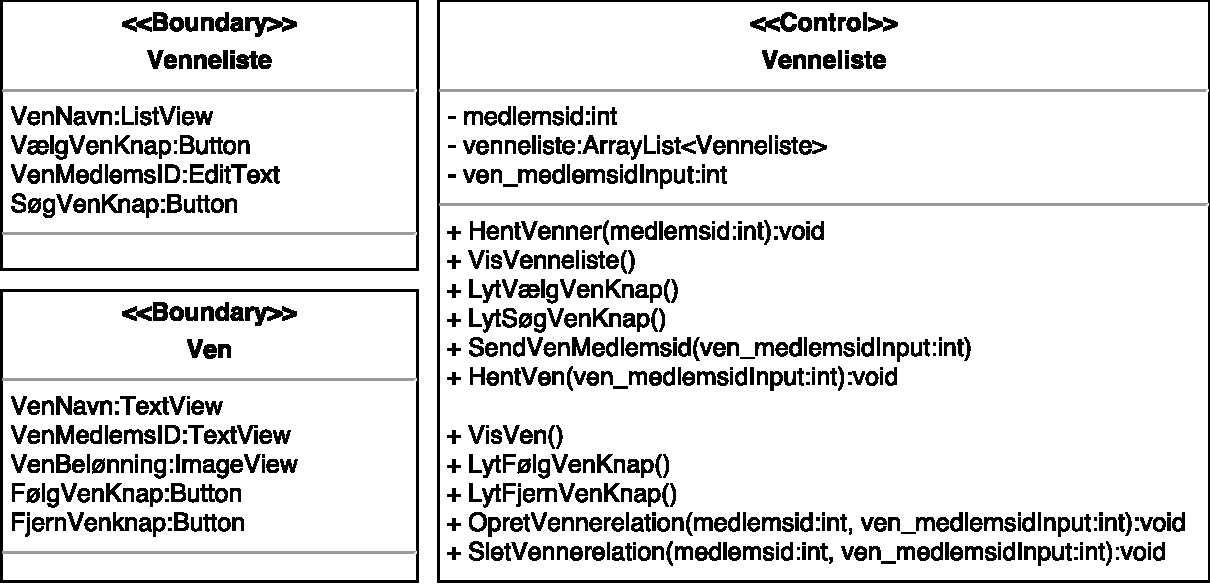
\includegraphics[width=1\textwidth]{figures/MVC/MVCVenneliste}
\caption{Designklasser for venneliste. Til venstre ses boundary for Venneliste og Ven, hvor der til højre ses tilhørende controller.}
\label{fig:MVCVenneliste}
\end{figure}

\noindent
I \textit{Venneliste}-grænsefladen findes en liste, af typen ListView, med navn på de brugere, der følges. Hver bruger, der vises af den givne grænseflade, kan tilgås ved at trykke på brugeren. Derudover er der i denne grænseflade et søgefelt, af typen EditText, med en tilhørende SøgVenKnap, af typen Button, som muliggør, at brugeren kan søge på andre brugere ved at angive deres medlemsID. 
\textit{Ven}-grænsefladen indeholder tekstfelter af typen TextView, som viser brugerens navn og medlemsID. Derudover er der anvendt billede af typen ImageView, som viser brugerens belønninger. Hvis brugeren ikke følges, er der her opstillet en FølgVenKnap. Følges brugeren allerede er der opstillet en FjernVenKnap. 

Controller for \textit{Venneliste} indeholder attributter, herunder attributter af typen int og ArrayList. Arrayet for venneliste har til formål at lagre brugerens venner. Dertil har controlleren ligeledes metoder, herunder Hent, Vis, Lyt, Søg, Valider, Opret og Slet. Metoderne handler ud fra inputsparametre angivet i parenteserne. 

Ud fra de nævnte designklasser er udarbejdet et sekvensdiagram, der fremgår af \autoref{fig:SEKVenneliste}.

\begin{figure} [H]
\centering
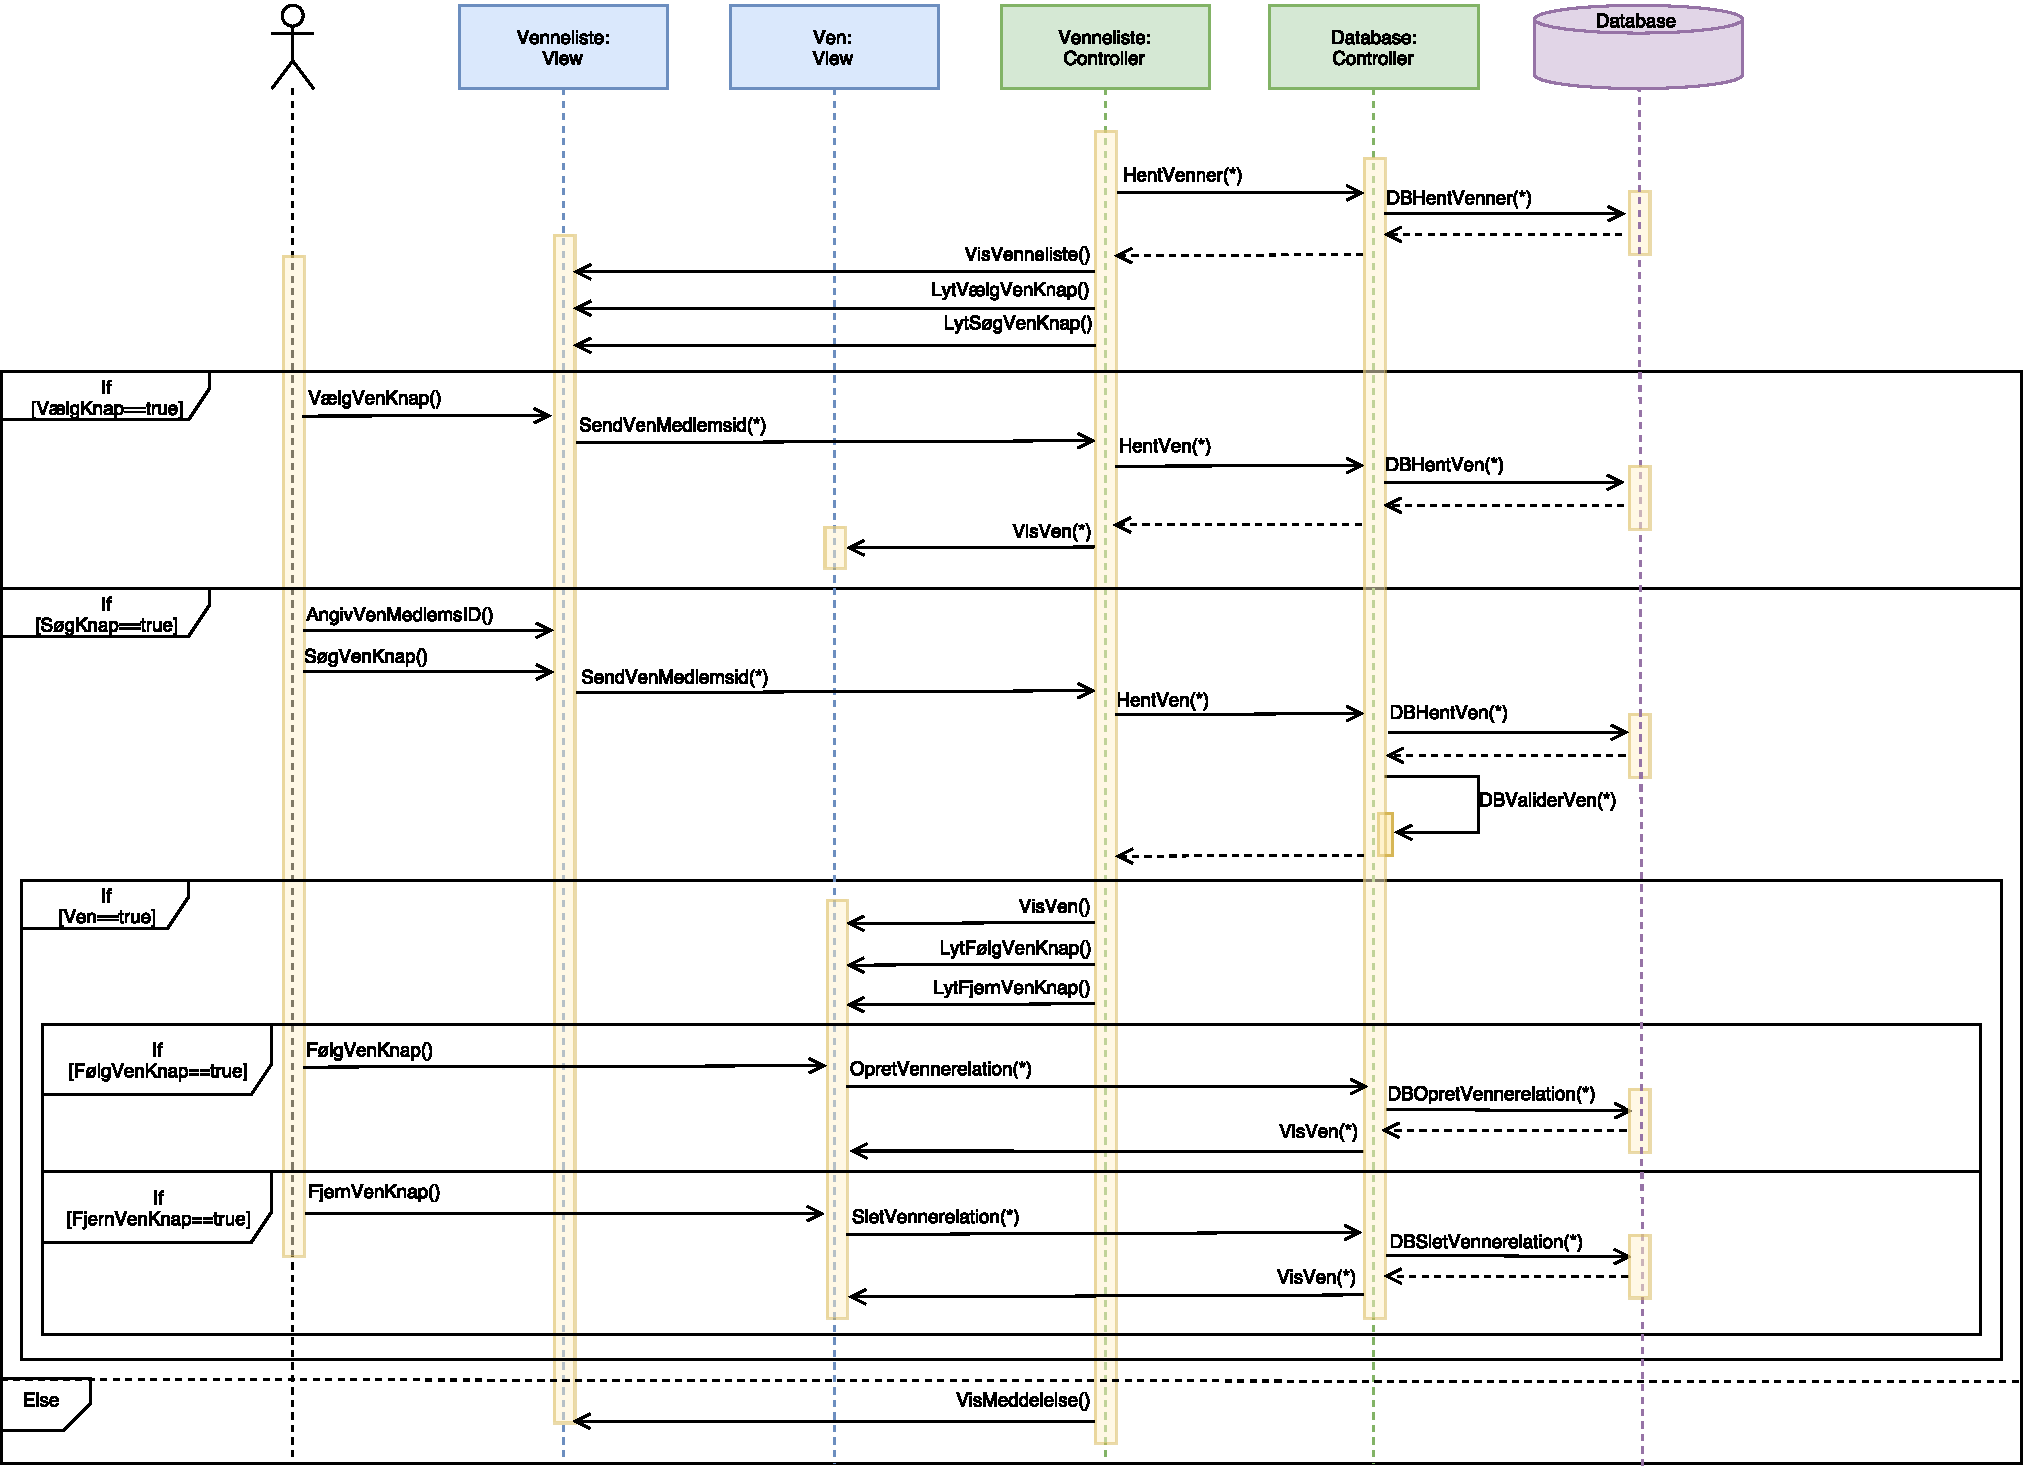
\includegraphics[width=1.55\textwidth, angle=90]{figures/Sek/SEKVenneliste}
\caption{Sekvensdiagram for venneliste.}
\label{fig:SEKVenneliste}
\end{figure}

\noindent
\textit{Venneliste}-controlleren henter venner fra \textit{Database} via \textit{Database}-controlleren, hvorefter grænsefladen for venneliste vises. 
Dertil lytter controlleren på VælgVenKnap samt SøgVenKnap. Vælger brugeren at tilgå en ven fra vennelisten, sendes vennens medlemsID til \textit{Venneliste}-controlleren, hvorefter vennen og vedkommendes belønninger hentes i databasen. Dertil vises grænsefladen for \textit{Ven}. Vælger brugeren derimod at søge efter en anden bruger, sendes det indtastede medlemsID, således den søgte bruger kan findes i databasen, hvortil den valideres. Såfremt brugeren ikke findes i databasen, vises en fejlmeddelelse i \textit{Venneliste}-grænsefladen. Findes brugeren i databasen, vises grænsefladen for \textit{Ven}, hvor brugeren har mulighed for at følge eller fjerne en bruger. Hvis brugeren trykker på FølgVenKnap oprettes der en vennerelation i databasen, hvor vennerelationen modsat vil slettes ved tryk på FjernVenKnap. Efterfølgende sendes en bekræftelse på, at vennen er tilføjet eller fjernet. 


%Venneliste inddeles i en grænseflade og dertilhørende controller, som det fremgår af \autoref{fig:MVCVenneliste}. 

%\begin{figure} [H]
%\centering
%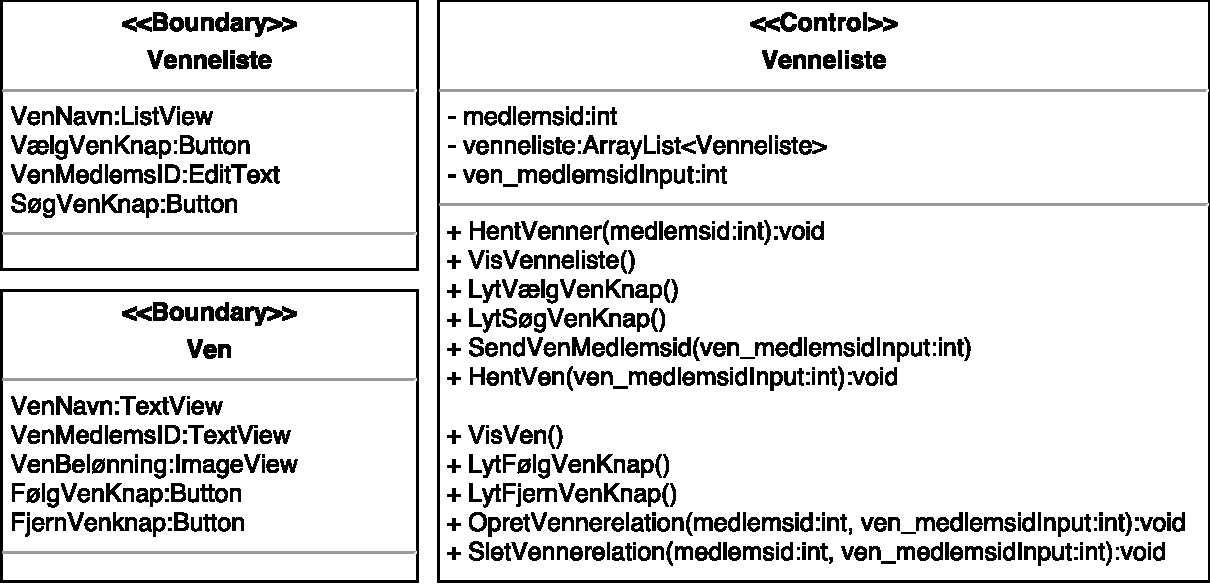
\includegraphics[width=0.8\textwidth]{figures/MVC/MVCVenneliste}
%\caption{Designklasser for venneliste.}
%\label{fig:MVCVenneliste}
%\end{figure}

%\noindent
%\textit{VennelisteGrænsefladen} indeholder tekstfelter for fornavn og efternavn på de brugere de følger. Derudover er der opstillet tekstfelt for medlemsID, hvor brugeren kan angive medlemsID'et på en bruger de ønsker at følge. Dertil er der opstillet en tilhørende søge knap, af typen button, der ved tryk indikere at brugeren har angivet medlemsID på brugeren den ønsker at følge. Derudover har brugeren mulighed for at vælge en bruger eller gå tilbage via en vælg eller tilbage  knap, der også er af typen button. 


%Der er til \textit{VennelisteGrænsefladen} opstillet en \textit{VennelisteController}, der har til formål at vise en oversigt over vennelisten når grænsefladen for vennelisten tilgås. Brugeren har via vælg knappen mulighed for at tilgå en bruger den følger
%Controlleren lytter på om brugeren trykker på vælg knappen eller søg knappen. Vælg knappen giver brugeren mulighed for at tilgå enkelt bruger ud fra vennelisten. Trykker brugeren på søg knappen kontrollere controlleren om det angivne medlemsID findes i databasen, herefter kan brugeren trykke på vælg. Trykkes der på en af vælg knapperne, enten i vennelisten eller efter søgning på medlemsID vises \textit{VenGrænsefladen}, som fremgår af \autoref{MVCVen}. Controlleren lytter på tilbage knappen, hvis denne trykkes på vises forrige grænseflade. 


%\subsubsection*{Ven}
%Ven inddeles i en grænseflade og tilhørende controller, som det fremgår af \autoref{fig:MVCVen}.

%\begin{figure} [H]
%\centering
%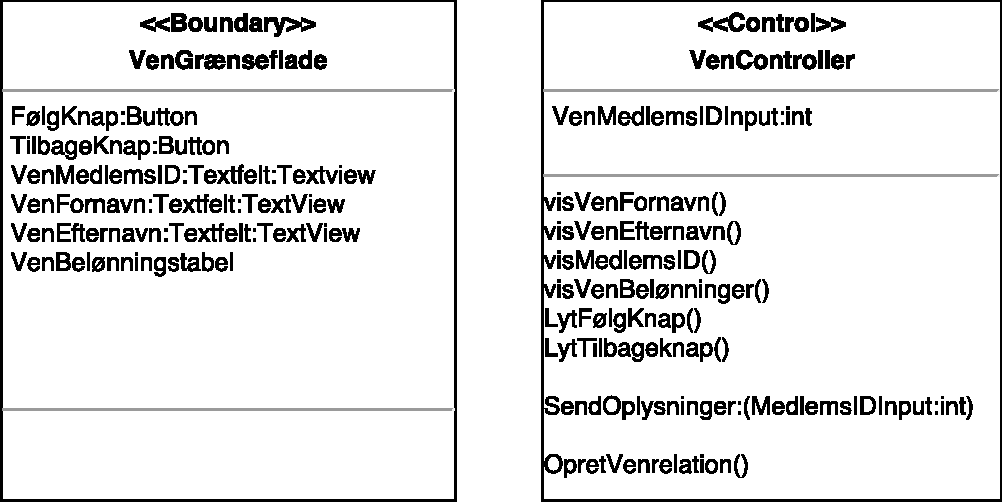
\includegraphics[width=0.8\textwidth]{figures/MVC/MVCVen}
%\caption{Designklasser for ven.}
%\label{fig:MVCVen}
%\end{figure}

%\noindent
%I \textit{VenGrænseflade} vises tekstfelter for valgt bruger, herunder MedlemsID, fornavn og efternavn. Dertil er der opstillet en følg knap og en tilbage knap af typen button. Følg knap er kun tilgængelig, hvis brugeren ikke følger den valgte ven. Derudover vises en tabel med den valgte brugers belønninger.


%Til \textit{VenGrænsefladen} er der opstillet en \textit{VenController}, som har til formål vise brugeroplysninger, herunder MedlemsID, fornavn og efternavn samt belønningstabel for den valgte bruger. Controlleren lytter på om brugeren trykker på følg knappen, hvis brugeren ikke allerede følger eller trykker på tilbage knappen. Trykkes der på følg knappen sendes MedlemsID'et på den bruger der ønskes at følges til databasen, hvorefter vennerelation gemmes i denne. Vælger brugeren at trykke på tilbage knappen vises den forrige grænseflade.   